\documentclass{ctexbeamer}
\usepackage{amsmath}
\usepackage{graphicx}
\usepackage{minted}
\usepackage{fontspec}
\usepackage{xcolor}
% \usepackage[colorlinks=true]{hyperref}

\usetheme{Madrid}
\usecolortheme[rgb={1,0,0}]{structure}
\definecolor{mintbg}{rgb}{0.95,0.95,0.95}
\setmonofont{WenQuanYi Micro Hei Mono}
\setbeamertemplate{background}{
\includegraphics[height=\paperheight]{pics/bg.png}}

\title{爱国者治港}
\subtitle{Patriots rule Hong Kong}
\author{
    711202 形政第七小组
}

\begin{document}
    \begin{frame}
        \maketitle
    \end{frame}

    \begin{frame}
        \frametitle{组员名单}
    
        \begin{center}
            \begin{itemize}
                \centering
                \item 71120218 张炎
                \item 71120219 张云杰
                \item 71120220 王致远
                \item 71120221 梁鹏明
                \item 71120222 王士翰
                \item 71120223 毛忠昊
                \item 71120224 文拳
                \item 71120225 吕天翼
                \item 71120226 陈宇轩
            \end{itemize}
        \end{center}
    
    \end{frame}

    \begin{frame}
        \frametitle{目录}
    
        \tableofcontents
    
    \end{frame}

    \section{背景}

    \begin{frame}
        \frametitle{背景}
        
        \begin{figure}
            \centering
            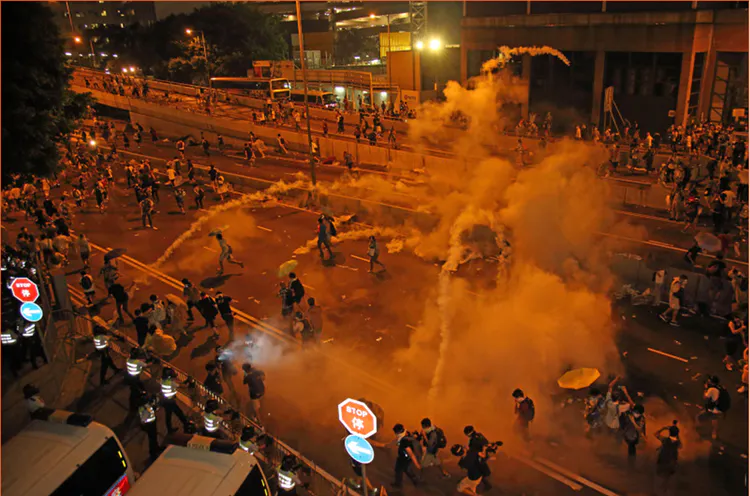
\includegraphics[scale=0.3]{pics/pic1.png}
            \caption{“香港占中事件”中街头的混乱场面}
        \end{figure}
    
    \end{frame}

    \begin{frame}
        \frametitle{背景}
    
        在过去20多年的时间里,香港特区不断出现各种各样新的情况和纷繁复杂的问题,屡屡出现严重的社会危机和管治危机,甚至是严峻的宪制危机,背离“一国两制”基本方针政策的初心,挑战“一国两制”实践的原则底线的作法时有发生。
    
    \end{frame}
\end{document}